\documentclass[runningheads,a4paper,fleqn]{llncs}

\usepackage{amsmath}
\usepackage{amssymb}
\usepackage{alltt}
\usepackage{lineno}
\usepackage{graphicx}
\usepackage[normalem]{ulem}

\usepackage{tikz}
\usetikzlibrary{arrows,petri,topaths}
\usepackage{tkz-berge}

\begin{document}

\title{Multi-Lane FlowPools: A detailed look}
\author{Tobias Schlatter\inst{1} \and Aleksandar Prokopec\inst{2} \and
  Heather Miller\inst{2} \and Philipp Haller\inst{2} \and Martin
  Odersky\inst{2}}

\authorrunning{Tobias Schlatter}

\institute{Student, EPFL \and Advisor, EPFL}

\maketitle

\begin{abstract}
  FlowPools, proposed by \cite{FP12} are a powerful way to express
  dataflow logic in highly parallelized applications. The original
  paper proposes two ways of implementing a FlowPool: Single-Lane
  FlowPools (SLFP) and Multi-Lane FlowPools (MLFP). While SLFPs are
  relatively simple to implement, insertions do not scale. MLFPs solve
  this limitation. This report goes into the details of the
  implementation of MLFPs and analyzes some benchmarking results in
  %% TODO what does it?
  more detail to show that insertions MLFPs scale nicely, with respect
  to SLFPs, and other concurrent data structures.
\end{abstract}

\section{Introduction}
The goal of this section is to briefly remind the reader of the
semantics and programming interface of a FlowPool and the basic ideas
behind the implementation of SLFPs to allow for better understanding
of the implementation of MLFPs.

\subsection{Programming Model}
The following operations are supported by a FlowPool. For a proof of
determinism, refer to \cite{FP12}.

\textbf{Append (\texttt{<<})} Inserts an element in the
FlowPool. Fails if the number of elements the FlowPool has been sealed
with is reached.\\
Signature: \verb+def <<(x: T): Unit+

\textbf{Foreach} Traverse elements in the FlowPool. Calls a closure
\verb+f+ exactly once (asynchronously) for each element added to the
FlowPool (until it is sealed). Returns future of number of elements in
pool. Foreach is normally implemented using the more general primitive
\verb+aggregate+.\\
Signature: \verb+def foreach[U](f: T => U):+ \verb+Future[Int]+

\textbf{Aggregate} Reduce elements in the FlowPool to a single
value. Starts off with \verb+zero+ as initial value to aggregate on,
calls \verb+op+ exactly once per element to add it to an aggregation,
finally uses \verb+cb+ to combine multiple aggregations into a single
one. Note that \verb+op+ is guaranteed to be executed only once per
element, whereas \verb+cb+ may be called any number of times\\
Signature: \verb+def aggregate[S]+\verb+(zero: =>S)+
\verb+(cb: (S, S) => S)+\\
\verb+(op: (S, T) => S):+ \verb+Future[S]+

\textbf{Builders} Abstraction to allow garbage collection of elements
that are no longer required. Allows insertion without reference to
initial pool (and hence all elements). See \cite{FP12} for details.

\textbf{Seal} Fixes the number of elements that will eventually be in
the pool allowing callbacks to be freed once reached. The final size
of the pool is required as argument in order to preserve the
determinism of the model. Subsequent call to \verb+seal+ will fail iff
the FlowPool has already been sealed with a different size or the
number of elements in the FlowPool is larger than the seal size.\\
Signature: \verb+def seal(size: Int): Unit+

\subsection{Single-Lane FlowPool}
SLFPs are implemented using a single linked-list of arrays of
elements, where the last non-empty element does not hold actual data,
but the state of the FlowPool, i.e. a list with all the callbacks and
the seal state of the FlowPool. Changes to the SLFP are only allowed
by CASing at this particular point, which hence serves as
linearization point of the datastructure.

With competing, concurrent writers, this approach does not scale
nicely (see figure~\ref{fig:eval-cpu-scaling}). Mainly due to cache
contention (multiple CPUs often write to close memory locations) and
CAS collisions.

\section{Implementation}
MLFPs take advantage of the lack of ordering guarantees in the
FlowPool semantics to remove the limitation of SLFPs with respect to
scaling by applying a simple but effective idea: Instead of having a
single SLFP, we use one SLFP (from now on called lane) for each
processor (or thread). This means, that on one hand, every processor
(or thread) gets its own lane to which it appends elements to,
avoiding CAS collisions and cache contetion. On the other hand, every
callback or aggregation has to be registered on each of these lanes
seperately and completing the callback future has to be externaly
syncrhonized.

In the following, the implementation of the FlowPool operations in the
MLFP are explained in detail. Please refer to
figure~\ref{fig:mlfp-pseudocode} for pseudocode of the operations.

\subsection{Callbacks}
When calling \verb+aggregate+ on a MLFP, the implementation has to
assure that a copy of this callback is known to every underlying lane
and that upon completion of the callbacks for every lane, the values
are aggregated in the final result and the future is completed. Note
that callback addition to a given lane is no different than in SLFPs.

The aggregation of each lane's final values is done using a FlowLatch,
a construct that allows aggregating a given number of values into a
single one using similar semantics as a FlowPool. A FlowLatch may
supply a future that is completed with the aggregated value, once the
expected number of values has been supplied. \verb+aggregate+ returns
this future to the caller.

\subsection{Seal}
The \verb+seal+ operation is the only one whose complexity increases
with multiple lanes, as the overall size guarantee has to be
established over all lanes while preserving lock-freedom and
linearizability, especially in the face of errors occuring while
sealing.

To ensure the latter, a global seal state (stored in a location common
to the whole MLFP) is required. The global seal may be in one of the
following states (state transition graph in
figure~\ref{fig:seal-states}):
\begin{itemize}
\item \verb+Unsealed+ (U): No seal has yet been attempted, or all
  seales have failed.
\item \verb+Proposition(size)+ (P): Sealing with given (total) size is
  being attempted. No other sealing operation may be attempted until
  this state is resolved to one of the other two. Threads attempting
  to seal and encountering a \verb+Proposition+ state, shall help the
  resolution of the state. (This is required to ensure lock-freedom)
\item \verb+Sealed(size, remain)+ (S): The MLFP has been sealed with
  size \verb+size+, where at the moment of the sealing, \verb+remain+
  free slots were remaining. The latter value is required to
  distribute the remaining element slots amongst the lanes and will be
  explained in detail later.
\end{itemize}

%% Seal-State transition graph
\begin{figure}
  \centering
  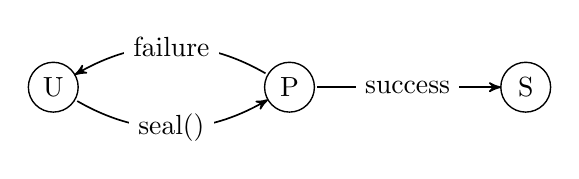
\begin{tikzpicture}[ node distance = 2cm ]
    \Vertex[x = 0, y = 0]{U}
    \Vertex[x = 3, y = 0]{P}
    \Vertex[x = 6, y = 0]{S}

    \tikzset{EdgeStyle/.style={post}}       % directed edges

    \Edge[label = success](P)(S)

    \tikzset{EdgeStyle/.append style = {bend right}}
    \Edge[label = {seal()}](U)(P)
    \Edge[label = failure](P)(U)

  \end{tikzpicture}
  \caption{State-transition graph of MLFP seal state}
  \label{fig:seal-states}
\end{figure}

Further, each lane holds its own seal state (similar to SLFPs) which
may be one of the following. The state transitions are the same as for
the global state (figure~\ref{fig:seal-states}).
\begin{itemize}
\item \verb+CallbackList+ (U): The lane is unsealed. A seal procedure
  might have been started but is not yet completed. Insertion may be
  handled as in a SLFP.
\item \verb+SealTag+ (P): A seal procedure has been started and any
  writer should resolve the tag by either helping to finish the
  sealing or replace it based on the global state.
\item \verb+Seal(size)+ (S): This lane has been sealed with the given 
  size.
\end{itemize}

In the following, the different parts of the sealing procedure are
explained in detail.

\textbf{Seal} When a thread calls \verb+seal()+ it first checks the
current state of the MLFP. If it is in unsealed state, it tries to
change the seal state to proposition and then continue with the
sealing. If the MLFP is already in proposition state, it helps
finishing the current seal. If the MLFP is in \verb+Sealed+ state, the
call succeeds or fails immediately, depending on whether the sizes are
the same or not.

\textbf{Help Sealing} Once the MLFP is in proposition state, any
thread attempting to seal (or inserting an element as we will see
later), will start propagating the proposition state to each lane. It
does this by placing the special token \verb+SealTag+ into the state
location of the given lane, using a similar procedure as the
\verb+seal()+ procedure of the SLFP.

A thread that tries to insert an element and encounters a
\verb+SealTag+ must resolve the tag before it can continue on
(explained later). This ensures that, once a \verb+SealTag+ has been
placed in a lane, its size does not change any more until the seal is
finished, which allows to calculate a snapshot of the total number of
elements in the MLFP. Note that during this procedure, one might also
find that the seal has been completed (when encountering a \verb+Seal+
in a lane). In such a case, the helping can be stopped prematurely.

Note that each \verb+SealTag+ holds the proposition it corresponds to,
as other seal tags might still be present from a failed attempt to
seal.

When a thread that succeeds in calculating the snapshot of the size,
it will then try to change the MLFP's state to sealed (or to unsealed,
if the number of elements is too big) and replace every occurence of
\verb+SealTag+ in the lanes by a \verb+Seal+.

\textbf{Resolution of seal tags} When a writer encounters a
\verb+SealTag+ it first checks the current global state. If it
indicates, that the seal operation corresponding to the \verb+SealTag+
is still going on, the writer helps sealing as described above, then
retries writing. If the global state indicates that the structure has
been sealed, the writer calculates the remaining slots for this lane
according to the following formula and then seals this lane.
\[ n_{seal} = n_{cur} + \frac{n_{remain}}{l_{total}} +
   1_{\{ l_{cur} < n_{remain} \bmod l_{total} \}} \]
If the writer finds that the current global state is unsealed or a
different proposition than in the tag, it removes the tag and
continues inserting normaly.

\textbf{Finalization} Some procedures that are required to invoke the
callback scheduling properly when sealing (i.e. ensuring the
finalization procedure of each callback is called exactly once) have
been omitted here for simplicity.

\subsection{Insertion}
Insertion into a MLFP happens the same way as into a SLFP, however,
the lane in which the element is to be inserted has to be chosen
first. For the choice of the lane we want to:
\begin{itemize}
\item Avoid collision between competing threads to a maximum.
\item Allow to change the thread-lane assignment, once some lanes have
  been entirely filled (after a seal).
\item Assure we can properly fill up the FlowPool entirely.
\end{itemize}
To achieve this, the following mapping is used at the beginning:
\[ l_{cur} = T_{cur} \bmod l_{total} \qquad
  (T_{cur} \text{ : Current thread ID}) \] 

When the first collision (i.e. attempted insertion into a full lane)
happens, the following hashed mapping is used:
\[ l_{cur} = \mathrm{rb}((T_{cur} + C) \cdot 9e3775cd_{16})
   \cdot 9e3775cd_{16}  \bmod l_{total} \]
where $C$ is the (global) number of collisions so far and
$\mathrm{rb}(\cdot)$ inverses the byte order.

After a certain number of collisions (currently the number of lanes),
the insertion switches to a linear search over all lanes to guarantee
that either the FlowPool is filled, or an error is raised due to too
many inserted elements.

Experimental results in figure~\ref{fig:lanef-scaling} show that there
is no use in having more than one lane per thread and hence that the
upper lane selection strategy is efficient. For further performance
evaluation of MLFPs, please refer to \cite{FP12}.

\begin{figure}[tbp]
  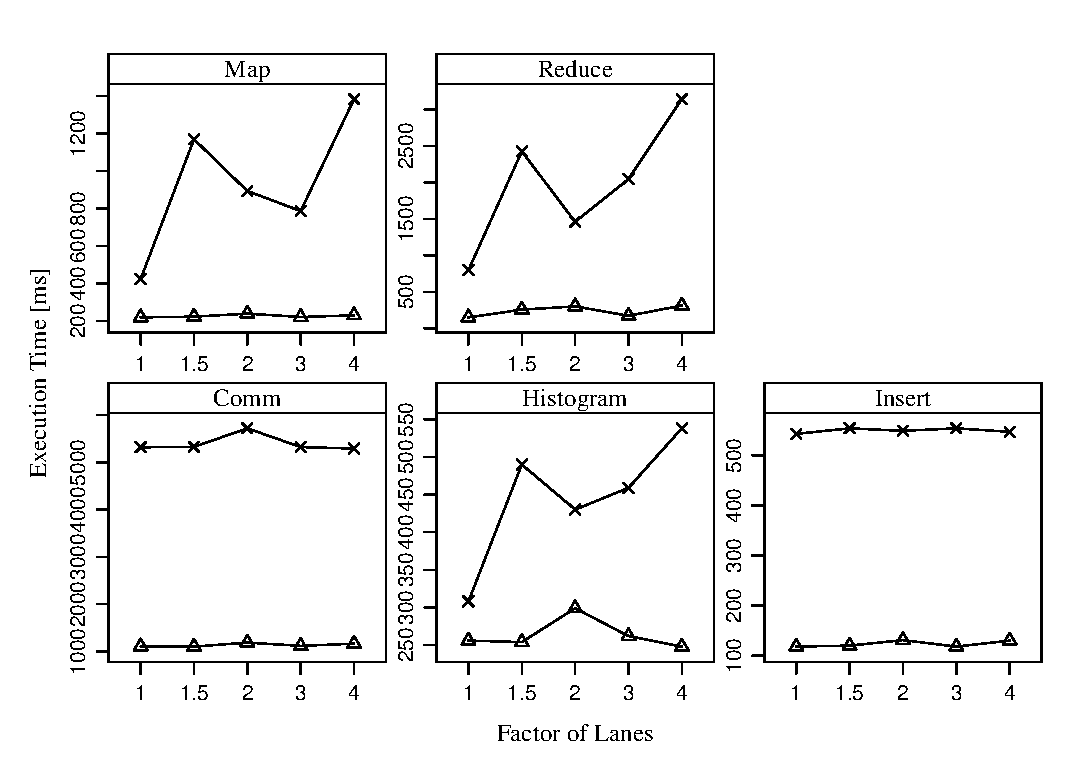
\includegraphics[width=\textwidth]{../../benchmarks/graphs/lanef-scaling}
  \caption{Execution times with respect to number of lanes per
    inserting thread in MLFPs. $\times$~UltraSPARC~T2,
    $\triangle$~4-core~i7}
  \label{fig:lanef-scaling}
\end{figure}

\begin{figure}

\centering

\begin{minipage}[b]{6cm}
\begin{alltt}
{\scriptsize
{\internallinenumbers{def aggregate[S](zero: =>S)
                (cmb: (S, S) => S)
                (folder: (S, T) => S):
    Future[S] = \{

  val aggregator = FlowLatch[S](zero)(cmb)
  aggregator.seal(laneCount)
    
  for (l <- lanes) \{
    l.registerCB(folder, zero, aggregator)
  \}
  
  aggregator.future
\}

def seal(size: Int) \{
  val cur_state = state
  cur_state match \{
    case Unsealed =>
      val ns = Proposition(size)
      if (!CAS(state, cur_state, ns))
        seal(size)
      else if (!helpSeal(ns)) failure()
    case p: Proposition =>
      if (helpSeal(p)) failure()
      else seal(size)
    case Sealed(sz,_) if size != sz =>
      failure("already sealed")
    case _ => // Done
  \}
\}

def tryResolveTag[T](t: SealTag[T]) \{
  cur_state match \{
    case p: Proposition if (p eq t.p) =>
      helpSeal(p)
    case Sealed(_,rem) =>
      val sz = sealSize(cur_state)
      writeSeal(Seal(sz))
    case _ => revertTag()
  \}
\}
}}}
\end{alltt}
\end{minipage}
\begin{minipage}[b]{6cm}
\begin{alltt}
{\scriptsize
{\internallinenumbers{def helpSeal(p: Proposition): Boolean = \{
  var sizes: Int = 0

  for (l <- lanes) \{
    writeSealTag(l, p) match \{
      case OnGoing(v)   =>
        sizes = sizes + v
      case Finished(success) => return success
    \}
  \}

  if (sizes <= p.size) \{
    // Seal MUST succeed
    val remaining = p.size - sizes
    val ns = Sealed(p.size, remaining)
    if (CAS(state, p, ns))
      finalizeSeals(remaining)
    true
  \} else \{
    // Seal MUST fail
    CAS(state, p, Unsealed)
    false
  \}

\}

def append(x: T) \{
  val index = \{
    if (collisions <= 0)
      curTID % laneCount
    else if (collisions <= laneCount)
      hash(curTID, collisions)
    else
      findEmptyLane() // Fails if not found
  \}

  if (!lanes(index).append(x)) \{
    increment(collisions)
    append(x)
  \}

\}
}}}
\end{alltt}
\end{minipage}

\caption{Multi-Lane FlowPool operations pseudocode}
\label{fig:mlfp-pseudocode}

\end{figure}

\begin{figure}
\centering
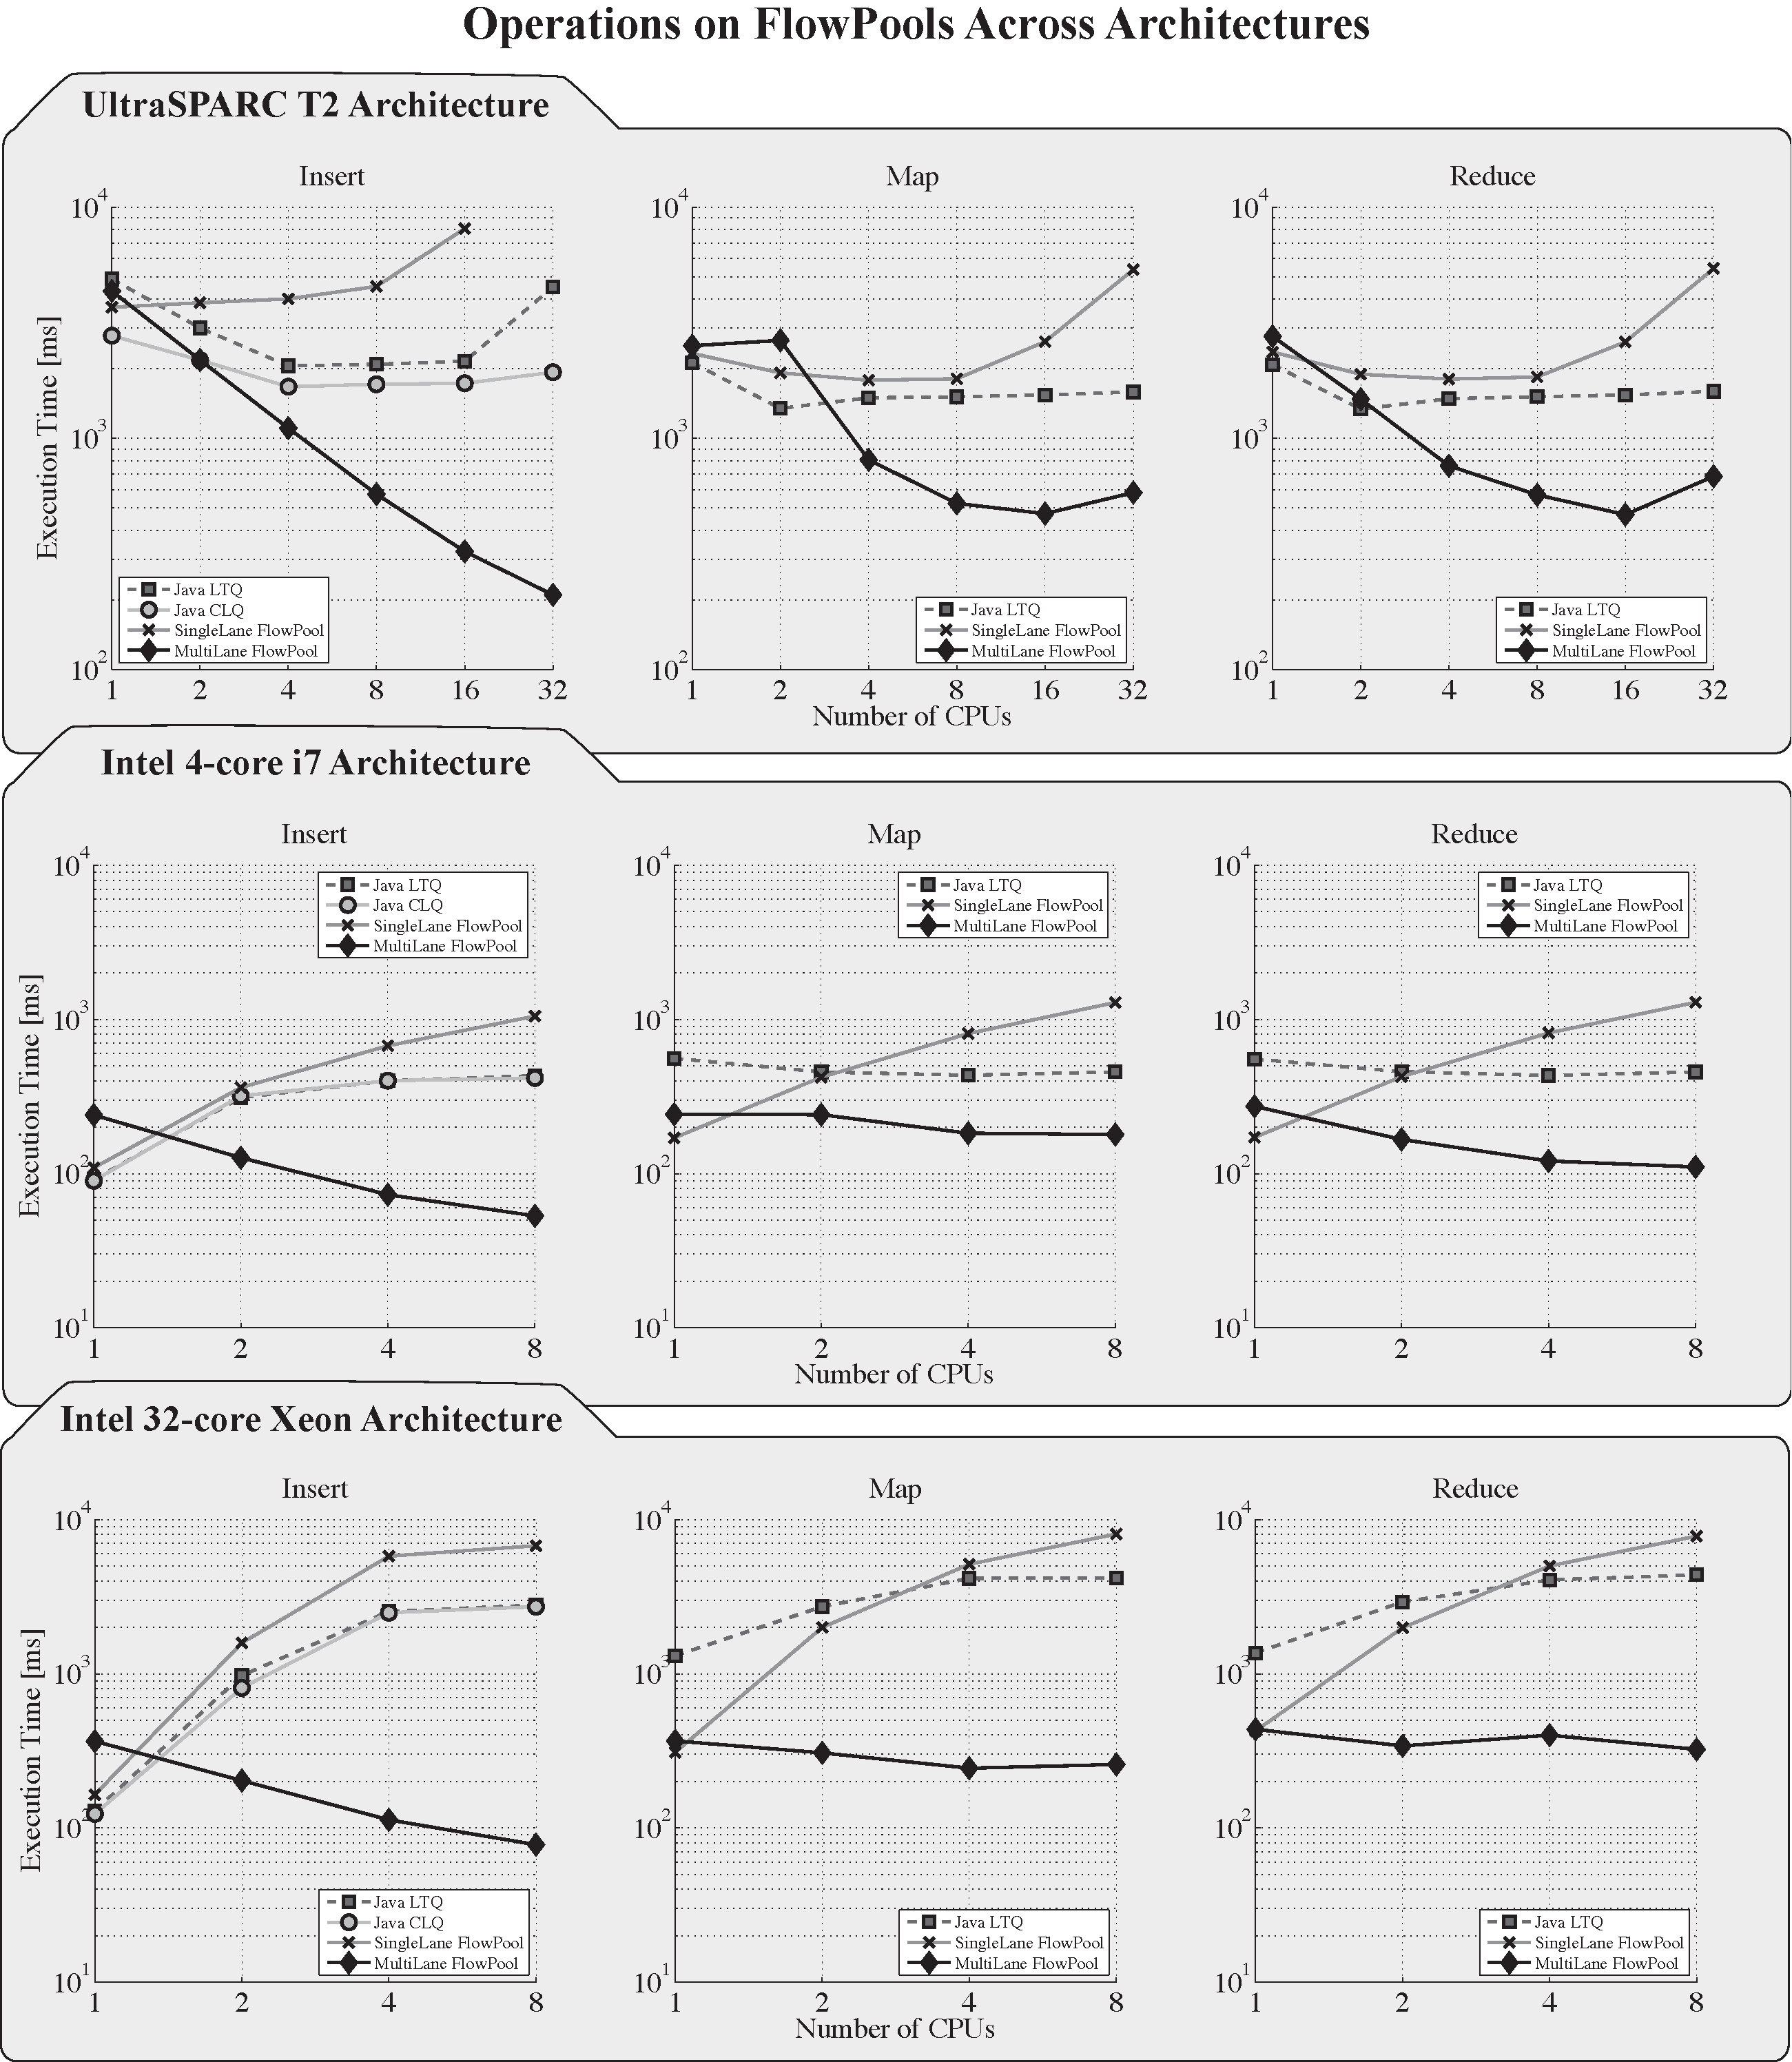
\includegraphics[width=\textwidth]{../../benchmarks/graphs/scaling-operations}
\caption{Execution time vs parallelization across three different
  architectures on three important FlowPool operations; insert, map,
  reduce.}
\label{fig:eval-cpu-scaling}
\end{figure}

\begin{figure}
\centering
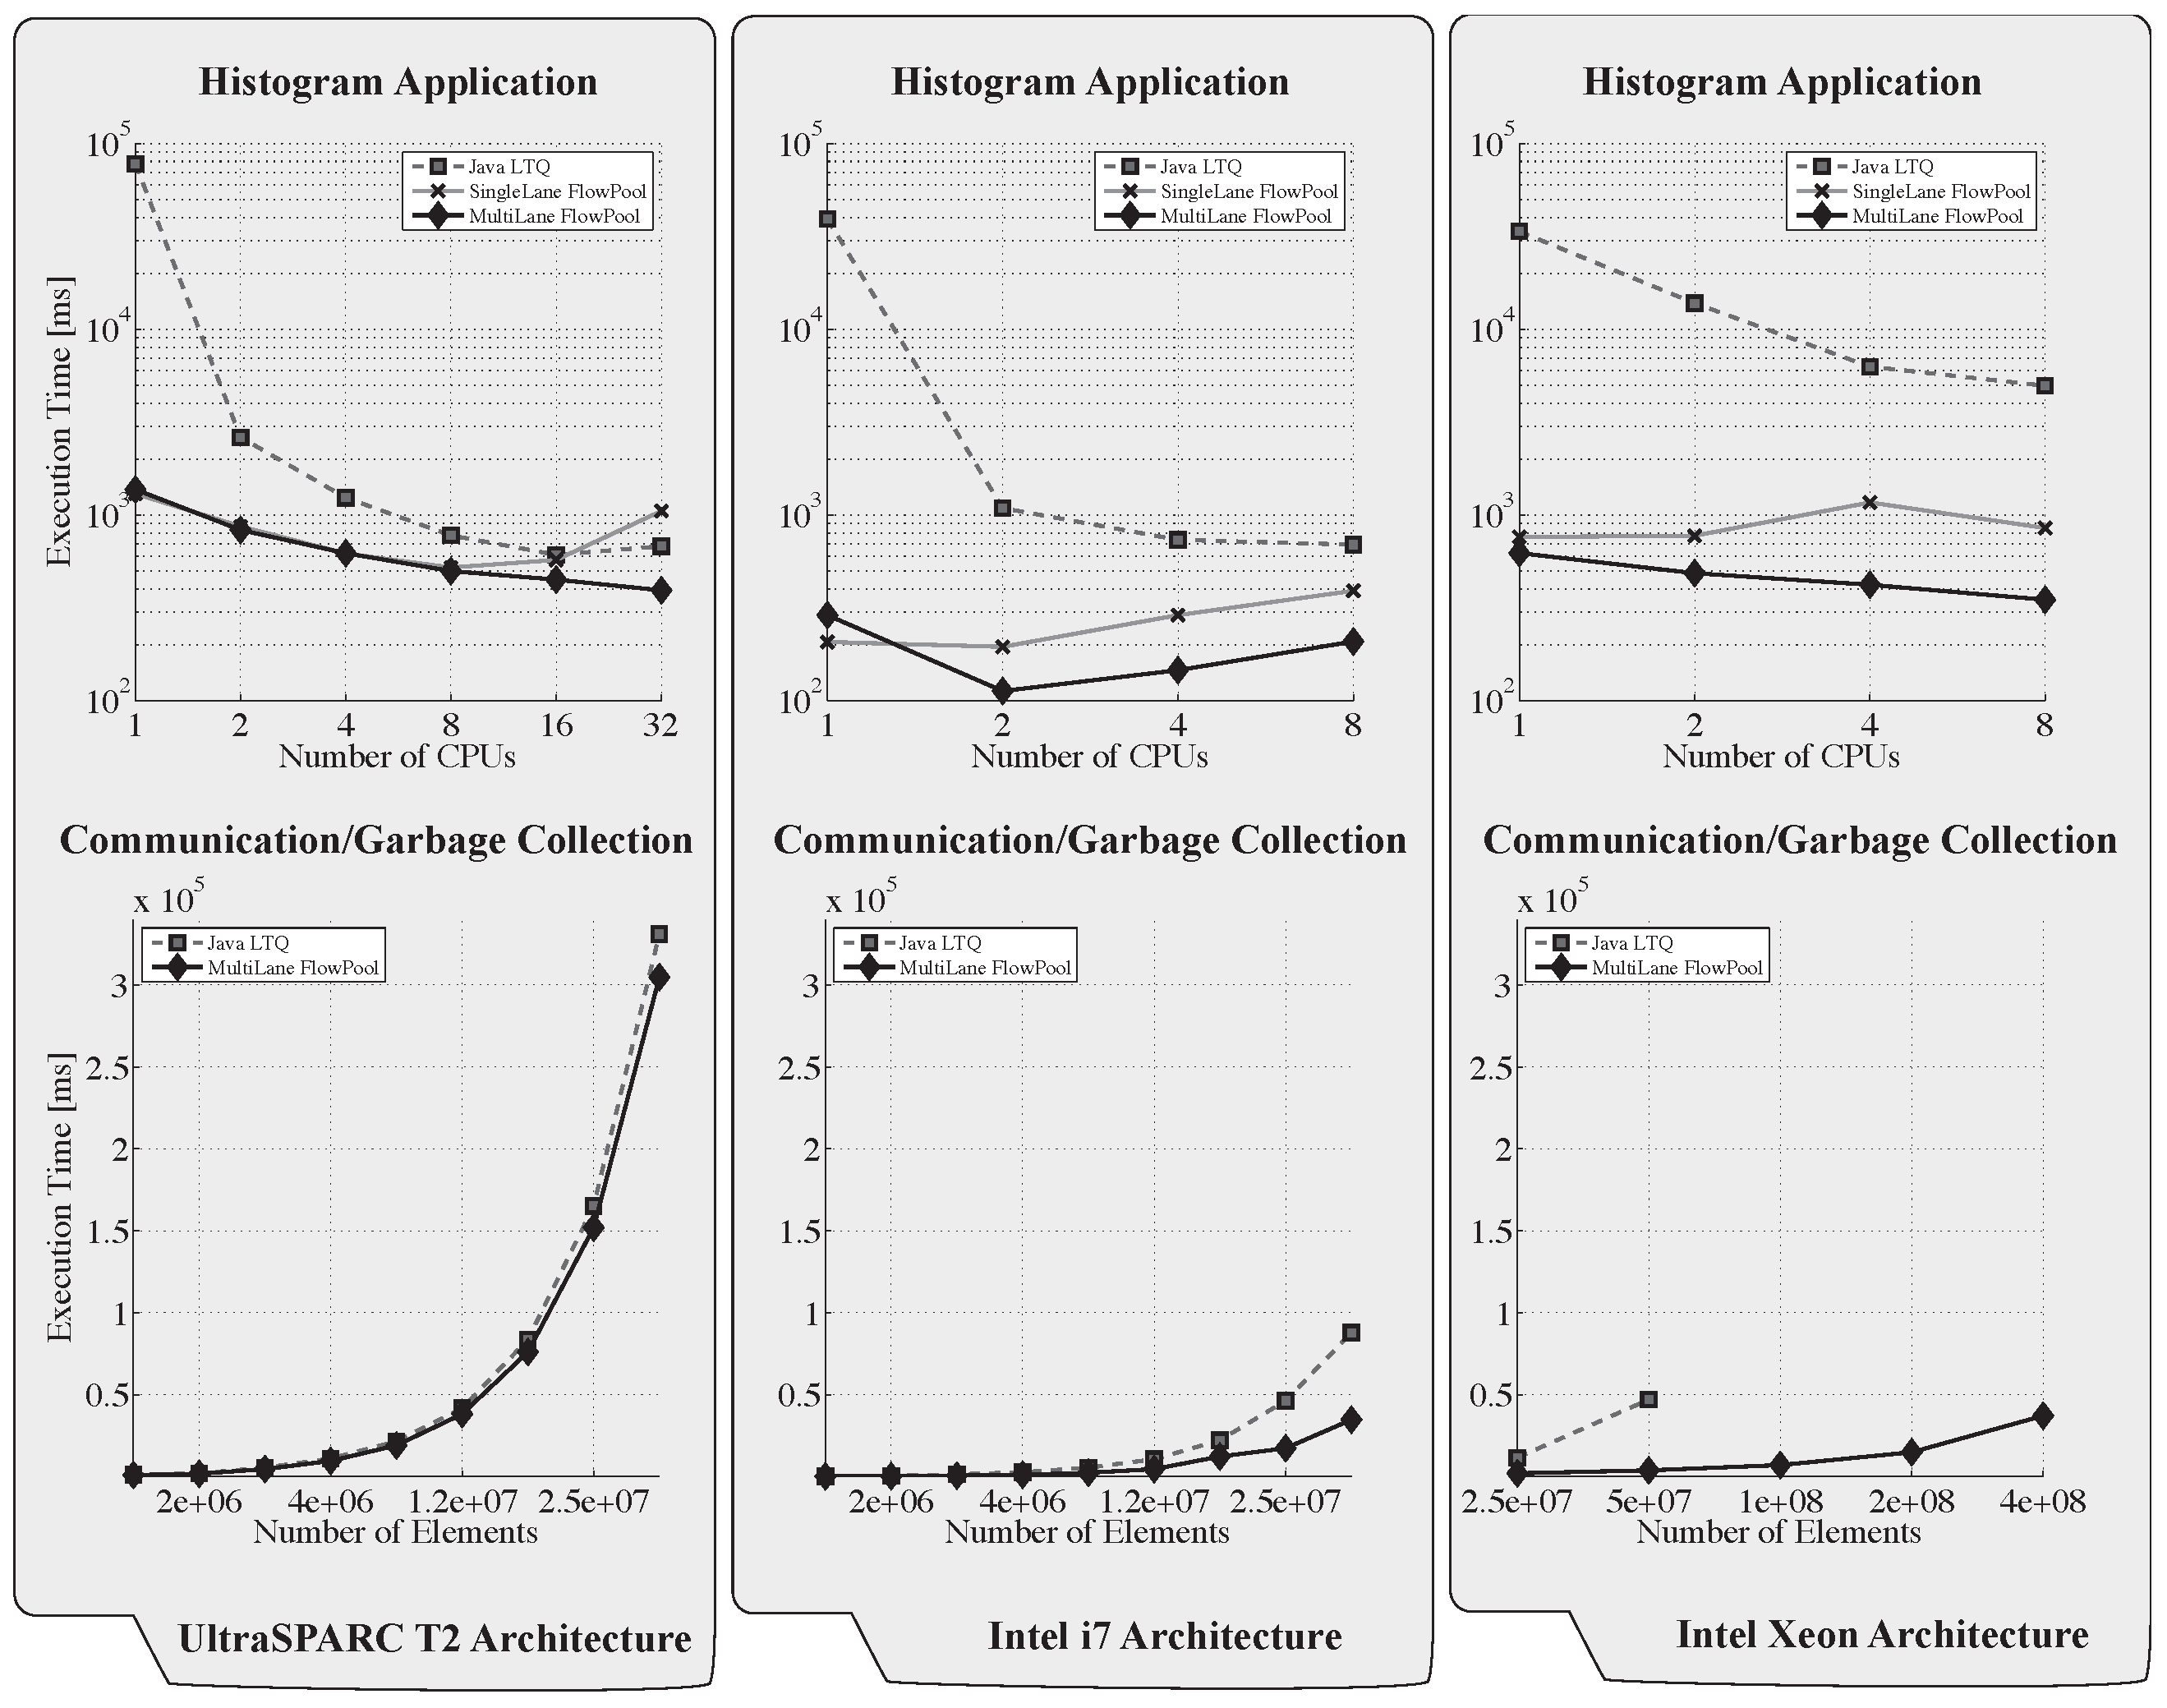
\includegraphics[width=\textwidth]{../../benchmarks/graphs/hist-comm}
\caption{Execution time vs parallelization on a real histogram application
(top), \& communication benchmark (bottom) showing memory efficiency, 
across all architectures.}
\label{fig:eval-hist-comm}
\end{figure}

\section{Correctness}
This section uses the notation, definitions and results from
\cite{FP12} and extends the proofs given there to an outline of a
correctness proof of MLFPs.

\begin{definition}[Taggable abstract pool]
  A taggable abstract pool is an abstract pool, except that
  \[ seal \in \{ -2, -1 \} \cup \mathbb{N}_0 \]
\end{definition}

\begin{definition}[Taggable abstract pool operations]
  A taggable abstract pool supports all operations of an abstract pool
  and in addition:

  Operation $tag()$, changes state from $(elems, cbs, -1)$ to $(elems,
  cbs, -2)$. Operation $untag()$, changes state from $(elems, cbs,
  -2)$ to $(elems, cbs, -1)$. In addition, no $append(\cdot)$ may be
  performed while $seal = -2$ and $seal(\cdot)$ may only be performed
  in states $(elems, cbs, -2)$.
\end{definition}

\begin{lemma}[MLFP Lanes]
  Each lane of a MLFP is consistent with an taggable abstract
  pool. (No proof given).
\end{lemma}

\begin{theorem}[Safety]
  Given a MLFP with lanes $L = \{l_1, \ldots, l_N\}$ each one being
  consistent with the taggable abstract pools $(elems_i, cbs_i,
  seal_i)$, the MLFP operations \verb+append+, \verb+foreach+ and
  \verb+seal+ are consistent with the abstract pool $(elems, cbs,
  seal)$, where 
  \[ elems = \bigcup_{i=1}^N elems_i \qquad
     cbs = \bigcap_{i=1}^N  cbs_i \]
\end{theorem}

\begin{theorem}[Linearizability]
  MLFP operations \verb+append+ and \verb+seal+ are linearizable.
\end{theorem}

\section{Conclusion}
In this report we have shown that a FlowPool as proposed by
\cite{FP12} can be implemented in a scalable way by using multiple
single-lane FlowPools. Further, we have provided a detailed
description including pseudo-code of how a multi-lane FlowPool is
implemented, especially with respect to sealing -- which has to be
fundamentally changed -- and the lane assignment rehashing strategy,
that does not exist in single-lane FlowPools. We used and included
benchmark results from the original paper to show that the proposed
rehashing strategy is efficient for a number of lanes equal to the
number of inserting threads.
%% TODO correctness proof?

\bibliographystyle{abbrv}
\bibliography{bib}

\end{document}

%%% Local Variables: 
%%% mode: latex
%%% TeX-master: t
%%% End: 
